\documentclass{article}
\usepackage[utf8]{inputenc}
\usepackage[margin=1in]{geometry}
\usepackage{amsmath, amsfonts}
\usepackage{fancyhdr}
\usepackage{multicol}
\usepackage{graphicx}
\usepackage[inline]{enumitem}
\graphicspath{ {images/} }
\pagestyle{empty}
\fancyhf{}
\cfoot{\thepage}
\pagenumbering{gobble}

\lhead{MATB42: Assignment \#7}
\rhead{
Poon, Keegan\\
1002423727\\
Mar 13th 2018}
\newcommand{\norm}[1]{\| #1 \|}
\newcommand{\deriv}[1]{\frac{d}{d #1}}
\newcommand{\parti}[1]{\frac{\partial}{\partial #1}}
\renewcommand{\headrulewidth}{0pt}
\newcommand{\gam}{\boldsymbol{\gamma}}
\begin{document}

\thispagestyle{fancy}

\begin{enumerate}
    \item
    \begin{enumerate}
        \item Find an equation of the tangent plane to the surface $S$ defined parametrically by $\boldsymbol \Phi(u, v) = (u^2 + v,\ v,\ u+v^2)$ at the point (9,0,3).
        \begin{align*}
            &v = 0 & &u + v^2 = 3 \implies u = 3&
        \end{align*}
        \begin{align*}
            \boldsymbol \phi_u &= (2(3), 0, 1) \\
            \boldsymbol \phi_v &= (1,1,2(0)) \\
            \boldsymbol \phi_u \times \boldsymbol \phi_v &= (-1,1,6) \\
        \end{align*}
        So the tangent plane can be given by
        \begin{align*}
            0 &= ((x - 9, y, z - 3) \cdot (-1,1,6)) \\
            0 &= (9 - x + y + 6z - 18) \\
            9 &= -x + y + 6z \\
        \end{align*}
        \item Use symbolic algebra software to sketch the surface $S$ and its tangent plane from part (a).
        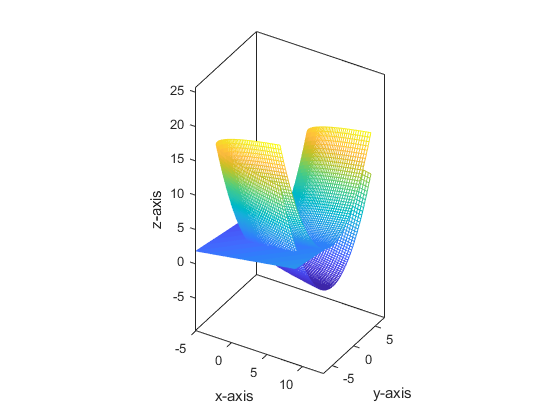
\includegraphics[width=\textwidth]{b42-a7-1b}
    \end{enumerate}

    \item Use a surface integral to find the area of the triangle in $\mathbb{R}^3$ with vertices (1,1,0), (1,2,1) and (3,3,2).

    \item Calculate the surface area of the piece of the cone $x^2+y^2-z^2 =0$ which lies inside the cylinder $x^2 + y^2 = 4$.
    
    We can see the radius of the cylinder is 2, so the cone portion that's cut out is the part which has radius less than or equal to 2 $\implies 0 \leq z \leq 2$. Using polar for the cone, $0 \leq \theta \leq 2 \pi$.
    \begin{multicols}{2}
    \noindent
    \begin{align*}
        \boldsymbol \Phi (\theta, z) &= (z\cos \theta, z\sin \theta, z) \\
        \boldsymbol \phi_\theta &= (- z \sin \theta, z \cos \theta, 0) \\
        \boldsymbol \phi_z &= ( \cos \theta, \sin \theta, 1) \\
        \boldsymbol \phi_\theta \times \boldsymbol \phi_z &= (z \cos \theta, z \sin \theta, - z \sin^2 \theta - z \cos^2 \theta) \\
        &= (z \cos \theta, z \sin \theta, - z)  \\
        \norm {\boldsymbol \phi_\theta \times \boldsymbol \phi_z }&= z^2 \cos^2 \theta + z^2 \sin^2 \theta + z^2  = 2 z^2\\
    \end{align*}
    \begin{align*}
        \int_{\boldsymbol \Phi} f \, dS &= \int_0^{2\pi} \int_0^2 2z^2 \, dz \, d\theta \\
        &= \int_0^{2\pi} \Big[ \frac{2}{3}z^3\Big]_0^2 \, d\theta \\
        &= \int_0^{2\pi} \frac{16}{3} d\theta =\frac{32\pi}{3} \\
    \end{align*}
    \end{multicols}
    \item
    \begin{enumerate}
        \item Find the area of the portion of the unit sphere that is cut out by the cone $z = \sqrt{x^2+y^2}$.
        \[ \Phi_{\text{sphere}} (\theta, \varphi) = (\cos \theta \sin \varphi, \sin \theta \sin \varphi, \cos \varphi) \]
        \[ \Phi_{\text{cone}} (\theta, z) = (z\cos \theta , z\sin \theta, z) \]

        (cf. page 391, \#10)

        \item Find the area of the portion of the cone $z = \sqrt{x^2+y^2}$ that is cut out by the unit sphere.
    \end{enumerate}

    \item Let $\boldsymbol \Phi : D \subset \mathbb{R}^2 \rightarrow \mathbb{R}^3$ be a parametrization of a 2-dim surface $S$ in $\mathbb{R}^3$.
    \begin{enumerate}
        \item Set
        \begin{align*}
            & E = \norm{\boldsymbol \phi_u}^2,& &F = \boldsymbol \phi_u \cdot \boldsymbol \phi_v, & & G = \norm{\boldsymbol \phi_v}^2,
        \end{align*} 
        Show that the surface area of $S$ is 
        \[ A(S) = \iint_D \sqrt{EG - F^2}\,dA \]
        
        \begin{align*}
            \iint_D \sqrt{EG - F^2}\,dA &= \iint_D \sqrt{\norm{\boldsymbol \phi_u}^2 \norm{\boldsymbol \phi_v}^2 - (\boldsymbol \phi_u \cdot \boldsymbol \phi_v)^2} \, dA \\
            &= \iint_D \sqrt{(\norm{\boldsymbol \phi_u}\norm{\boldsymbol \phi_v})^2 - (\norm{ \boldsymbol \phi_u} \norm{\boldsymbol \phi_v})^2 \cos^2\theta }\, dA & \text{Where $\theta$ is the angle between $\boldsymbol \phi_u$ and $\boldsymbol \phi_v$.}\\
            &= \iint_D \sqrt{(\norm{\boldsymbol \phi_u}\norm{\boldsymbol \phi_v})^2 (1 - \cos^2\theta) } \, dA \\
            &= \iint_D \sqrt{(\norm{\boldsymbol \phi_u}\norm{\boldsymbol \phi_v})^2 (\sin^2\theta) } \, dA \\
            &= \iint_D \sqrt{\norm{\boldsymbol \phi_u \times \boldsymbol \phi_v} ^2} \, dA \\
            &= \iint_D \norm{\boldsymbol \phi_u \times \boldsymbol \phi_v} \, dA \\
            &= \int_{\boldsymbol \Phi} 1\, dS
        \end{align*} 
        \item What does the formula for $A(S)$ become if the vectors $\boldsymbol \phi_u$ and $\boldsymbol \phi_v$ are orthogonal?


        If the vectors are orthogonal, then the dot product is 0, so the equation reduces to 
        \[ A(S) = \iint_D \norm{\boldsymbol \phi_u} \norm{\boldsymbol \phi_v}\, dA \]
        \item Use parts (a) and (b) to compute the surface area of a sphere of radius $a$.

        (cf. Marsden \& Tromba, page 399, \# 23.)
        \begin{align*}
            \boldsymbol \Phi (\theta, \varphi) &= a(\cos \theta \sin \varphi, \sin \theta \sin \varphi, \cos \varphi) \\
            \boldsymbol \phi_\theta &= a(- \sin \theta \sin \varphi, \cos \theta \sin \varphi, 0) \\
            \boldsymbol \phi_\varphi &= a( \cos \theta \cos \varphi, \sin \theta \cos \varphi, -\sin \varphi) \\
            \norm{\boldsymbol \phi_\theta} &= a\sin \varphi, \: \: \: \norm{\boldsymbol \phi_\varphi} = a \\
            \implies A(S) &= a^2\int_0^{2\pi}\int_0^\pi \sin \varphi \, d\varphi \, d\theta \\
            &= a^2\int_0^{2\pi}\Big[- \cos \varphi \Big]_0^{\pi} \, d\varphi \, d\theta \\
            &= a^2\int_0^{2\pi}- (-1 - 1) \, d\varphi \, d\theta \\
            &= a^22\int_0^{2\pi}1 \, d\varphi \, d\theta \\
            &= 4\pi a^2\\
        \end{align*} 



    \end{enumerate}
    \item For each of the following surfaces $S$, sketch $S$ (using symbolic software) and evaluate the surface integral $\int_S f \, dS$, where $f(x,y,z) = x$.
    \begin{enumerate}
        \item $S$ is that part of the surface $y=4-x^2$ between $z = 0$ and $z = 1$, with $y\geq 0$.
        \[ y \geq 0 \implies 4 - x^2 \geq 0 \implies x^2 \leq 4 \implies |x| < 2 \]
        \begin{align*}
                \boldsymbol \Phi (x,z) &= (x, 4-x^2, z) \\
                \boldsymbol \phi_x &= (1,-2x,0) ,\: \boldsymbol \phi_z = (0,0,1) \\
                \boldsymbol \phi_x \times \boldsymbol \phi_z &= (-2x, -1, 0) \implies \norm{\boldsymbol \phi_x \times \boldsymbol \phi_z} = \sqrt{4x^2 + 1} \\
                \int_S fdS &= \int_0^1\int_{-2}^{2}x\sqrt{4x^2 + 1}\, dx\, dz
        \end{align*}
        The integrand is odd since $x$ odd and $\sqrt{4x^2 + 1}$ even, so the integral over $x$ is 0, making the entire integral 0.
        \item $S$ is the upper half of the unit sphere centered at the origin.

        Only the upper half so $0\leq \theta \leq 2\pi$ and $0 \leq \varphi \leq \pi/2$.
        \begin{align*}
            \boldsymbol \Phi (\theta, \varphi) &= (\cos \theta \sin \varphi, \sin \theta \sin \varphi, \cos \varphi) \\
            \boldsymbol \phi_\theta &= (- \sin \theta \sin \varphi, \cos \theta \sin \varphi, 0) \\
            \boldsymbol \phi_\varphi &= ( \cos \theta \cos \varphi, \sin \theta \cos \varphi, -\sin \varphi) \\
            \boldsymbol \phi_\theta \times \boldsymbol \phi_\varphi &= (-\cos\theta \sin^2\varphi, -\sin\theta \sin^2\varphi, - \sin^2\theta \sin\varphi \cos\varphi - \cos^2\theta \sin \varphi \cos \varphi) \\
            &= (-\cos\theta \sin^2\varphi, -\sin\theta \sin^2\varphi, - \sin\varphi \cos\varphi ) \\
            \norm{\boldsymbol \phi_\theta \times \boldsymbol \phi_\varphi} &= \sqrt{\cos^2\theta \sin^4\varphi + \sin^2\theta \sin^4\varphi + \sin^2\varphi \cos^2\varphi } \\
            &= \sqrt{\sin^4\varphi + \sin^2\varphi \cos^2\varphi } \\
            &= \sqrt{\sin^2\varphi } = \sin\varphi \\
            \int_{\boldsymbol \Phi}f\, dS &= \int_0^{\frac{\pi}{2}}\int_0^{2\pi} \cos\theta \sin^2\varphi \, d\theta \, d\varphi = 0
        \end{align*} 
        The integral is zero again since integrating $\cos\theta$ over a whole period is 0.
        \item $S$ is that part of the surface $x = \sin y$ with $0 \leq y \leq \pi$ and $0 \leq z \leq 2$.

        \begin{align*}
            \boldsymbol \Phi (y,z) &= (\sin y, y, z) \\
            \boldsymbol \phi_y &= (\cos y, 1, 0) \\
            \boldsymbol \phi_z &= (0,0,1) \\
            \boldsymbol \phi_y \times \boldsymbol \phi_z &= (1, -\cos y, 0) \\
            \norm{ \boldsymbol \phi_y \times \boldsymbol \phi_z } &= \sqrt{1 +  \cos^2 y} \\
            \int_{\boldsymbol \Phi}f\, dS &= \int_0^2 \int_0^{\pi} \sin y \sqrt{1 + \cos^2 y} \, dy \, dz \\
        \end{align*} 
    \end{enumerate}

    \item Find the mass of the metallic surface $S$ given by $\displaystyle z = 1 - \frac{x^2 + y^2}{2}$ with $0 \leq x \leq 1$, $0 \leq y \leq 1$, if the mass density at $(x,y,z) \in S$ is given by $m(x,y,z) = xy$.
\end{enumerate}
\end{document}
